%%
%% Automatically generated file from DocOnce source
%% (https://github.com/doconce/doconce/)
%% doconce format latex whitepaper.do.txt --minted_latex_style=trac --latex_admon=paragraph --no_mako
%%


%-------------------- begin preamble ----------------------

\documentclass[%
oneside,                 % oneside: electronic viewing, twoside: printing
final,                   % draft: marks overfull hboxes, figures with paths
10pt]{article}

\listfiles               %  print all files needed to compile this document

\usepackage{relsize,makeidx,color,setspace,amsmath,amsfonts,amssymb}
\usepackage[table]{xcolor}
\usepackage{bm,ltablex,microtype}

\usepackage[pdftex]{graphicx}

\usepackage[T1]{fontenc}
%\usepackage[latin1]{inputenc}
\usepackage{ucs}
\usepackage[utf8x]{inputenc}

\usepackage{lmodern}         % Latin Modern fonts derived from Computer Modern

% Hyperlinks in PDF:
\definecolor{linkcolor}{rgb}{0,0,0.4}
\usepackage{hyperref}
\hypersetup{
    breaklinks=true,
    colorlinks=true,
    linkcolor=linkcolor,
    urlcolor=linkcolor,
    citecolor=black,
    filecolor=black,
    %filecolor=blue,
    pdfmenubar=true,
    pdftoolbar=true,
    bookmarksdepth=3   % Uncomment (and tweak) for PDF bookmarks with more levels than the TOC
    }
%\hyperbaseurl{}   % hyperlinks are relative to this root

\setcounter{tocdepth}{2}  % levels in table of contents

% Tricks for having figures close to where they are defined:
% 1. define less restrictive rules for where to put figures
\setcounter{topnumber}{2}
\setcounter{bottomnumber}{2}
\setcounter{totalnumber}{4}
\renewcommand{\topfraction}{0.95}
\renewcommand{\bottomfraction}{0.95}
\renewcommand{\textfraction}{0}
\renewcommand{\floatpagefraction}{0.75}
% floatpagefraction must always be less than topfraction!
% 2. ensure all figures are flushed before next section
\usepackage[section]{placeins}
% 3. enable begin{figure}[H] (often leads to ugly pagebreaks)
%\usepackage{float}\restylefloat{figure}

% prevent orhpans and widows
\clubpenalty = 10000
\widowpenalty = 10000

% --- end of standard preamble for documents ---


% insert custom LaTeX commands...

\raggedbottom
\makeindex
\usepackage[totoc]{idxlayout}   % for index in the toc
\usepackage[nottoc]{tocbibind}  % for references/bibliography in the toc

%-------------------- end preamble ----------------------

\begin{document}

% matching end for #ifdef PREAMBLE

\newcommand{\exercisesection}[1]{\subsection*{#1}}


% ------------------- main content ----------------------



% ----------------- title -------------------------

\thispagestyle{empty}

\begin{center}
{\LARGE\bf
\begin{spacing}{1.25}
Bachelor of Science program in Computational Physics and Quantum Technologies  at Department of Physics, UiO
\end{spacing}
}
\end{center}

% ----------------- author(s) -------------------------

\begin{center}
{\bf Morten Hjorth-Jensen and Anders Malthe-Sørenssen}
\end{center}

    \begin{center}
% List of all institutions:
\centerline{{\small Department of Physics and Center for Computing in Science Education, UiO}}
\end{center}
    
% ----------------- end author(s) -------------------------


% --- begin date ---
\begin{center}
Planned start: Fall 2024 (?)
\end{center}
% --- end date ---

\vspace{1cm}


\subsection*{Bachelor of Science program in Computational Physics and Quantum Technologies}

We would like to propose a new Bachelor of Science program at the
Department of Physics of the University of Oslo. This program is
called \textbf{Computational Physics and Quantum Technologies}, with acronym
\textbf{CPQT}. Tentative start fall semester 2024.
The program will be administrated by the Department of Physics. 

Possible collaborations with:

\begin{itemize}
\item Department of Chemistry

\item Department of Informatics

\item Department of Mathematics
\end{itemize}

\noindent
\subsection*{Strategic importance}

Computational physics, computational science and data science play a
central role in scientific investigations and are central to
innovation in most domains of our lives. These fields underpin the
majority of today's technological, economic and societal feats. We
have entered an era in which huge amounts of data offer enormous
opportunities, but only to those who are able to harness them. The 3rd
industrial revolution will alter significantly the demands on the
workforce. In particular, the developments taking place in quantum
technologies and quantum information systems (QIS) together with
artificial intelligence (AI) and machine learning (ML) are expected to
play a significant role in technology developments and innovations,
and for fundamental discoveries in physics.

\paragraph{AI and machine learning.}
Artificial
intelligence is built upon integrated machine learning algorithms,
which in turn are fundamentally rooted in optimization and statistical
learning.

Artificial intelligence (AI) and Machine learning (ML)  techniques
have in the last years gained considerable traction in
scientific discovery. In particular, applications and techniques for
so-called \textbf{fast ML}, that is high-performance ML methods applied
to real time experimental data processing, hold great promise for
enhancing scientific discoveries in many different disciplines.
These developments cover a broad mix of rapidly
evolving fields, from the development of ML techniques to computer and
hardware architectures.

An important and emerging field is what has been dubbed as scientific ML, see the article by Deiana et al \href{{https://arxiv.org/abs/2110.13041}}{Applications and Techniques for Fast Machine Learning in Science, arXiv:2110.13041}

The authors discuss applications and techniques for fast machine
learning (ML) in science -- the concept of integrating power ML
methods into the real-time experimental data processing loop to
accelerate scientific discovery. The report covers three main areas

\begin{enumerate}
\item applications for fast ML across a number of scientific domains;

\item techniques for training and implementing performant and resource-efficient ML algorithms;

\item and computing architectures, platforms, and technologies for deploying these algorithms.
\end{enumerate}

\noindent
For our research in for example particle and
nuclear physics, fields which cover a huge range of energy and length scales,
spanning from our smallest constituents to the physics of dense
astronomical objects like supernovae and neutron stars, AI and ML
techniques offer possibilities for new discoveries and deeper insights
about the physics of atomic nuclei, elementary particles and dense
matter. Similarly, ML algorithms are widely applied in condensed
matter physics, materials science and nanotechnology, in molecular dynamics simulations of complex
systems in neuroscience and in many other fields in natural science.

Examples of applications in subatomic physics
\begin{enumerate}
\item \textbf{Artificial Intelligence and Machine Learning in Nuclear Physics}, Amber Boehnlein et al., \href{{https://arxiv.org/abs/2112.02309}}{arXiv:2112.02309} and Reviews of Modern Physics, 2022, in press

\item \textbf{Predicting Solid State Material Platforms for Quantum Technologies}, Hebnes et al,. \href{{https://arxiv.org/abs/2203.16203}}{arXiv:2203.16203}

\item \href{{https://arxiv.org/abs/1803.08823}}{Mehta et al.} and \href{{https://www.sciencedirect.com/science/article/pii/S0370157319300766?via%3Dihub}}{Physics Reports (2019)}.

\item \href{{https://link.aps.org/doi/10.1103/RevModPhys.91.045002}}{Machine Learning and the Physical Sciences by Carleo et al}

\item \href{{https://pdg.lbl.gov/2021/reviews/rpp2021-rev-machine-learning.pdf}}{Particle Data Group summary on ML methods}
\end{enumerate}

\noindent
\paragraph{Quantum Information Technologies (QIT).}
Recent developments in quantum information systems
and technologies offer the possibility to address some of the most
challenging large-scale problems, whether they are represented by
complicated interacting quantum mechanical systems or classical
systems.  Originally proposed by Feynman, the efficient simulation of
for example quantum systems by other, more controllable quantum
systems formed the basis for modern constructions of quantum
computations.  Many algorithmic and theoretical advances have followed
since the initial work in this area and with recent developments in
quantum computing hardware there is an additional drive to identify
early practical problems on which these devices might demonstrate an
advantage.

In addition to theoretical activities conducted at the
Department of Physics (mainly at the Center for Computing in Science
Education (CCSE) and the condensed matter group and other groups), there is a growing
interest to study candidate systems for making quantum hardware. In
particular, so-called point defects in semiconductors are pursued by
experimenters at the center for Materials Science.  With this broad
list of activities at the department of physics, there is a huge
potential to prepare the ground for educating physicists with the
theoretical and experimental background needed for the 21st
century. There is also a great interest in candidates with such a
background, knowledge, skills and competences in industry and the
public sector.

\paragraph{Why such a program?}
Establishing such an educational program will be unique in Norway and
has the potential to attract excellent students.  The popularity of
the Computational Science and in particular the Computational Physics
and Computational Materials Science study direction are clear
indicattors that these are fields with the potential to attract new
students.

Furthermore,
Oslo Metropolitan university  has recently acquired two quantum quantum computers, see \href{{https://kommunikasjon.ntb.no/pressemelding/oslomet-avduker-norges-forste-kvantedatamaskin?publisherId=15678779&releaseId=17917781}}{\nolinkurl{https://kommunikasjon.ntb.no/pressemelding/oslomet-avduker-norges-forste-kvantedatamaskin?publisherId=15678779&releaseId=17917781}} and is now establishing research and educational initiatives in quantum information systems. There are thus several interesting avenues for joint collaborations in quantum information systems and quantum technologies as well as developing joint educational programs.

% !split
\subsection*{Links of interest to other (mainly MSc and PhD level) programs}

\href{{https://thequantuminsider.com/2022/06/06/top-20-quantum-computing-masters-ph-d-programs-in-2022/}}{List over top 20 quantum computing graduate programs (master of science and PhD programs) in 2022}

\begin{enumerate}
\item \href{{https://www.math.ku.dk/english/about/news/quantum-information-science-programme/}}{University of Copenhagen}

\item \href{{https://thequantumhubs.com/epfl-offers-a-new-master-in-quantum-science-and-engineering/}}{EPFL Lausanne}

\item \href{{https://quantummasterbarcelona.eu/}}{University of Barcelona}

\item \href{{https://master-qe.ethz.ch/}}{ETH Zurich}

\item \href{{https://qtom.qtedu.eu/}}{Quantum Technology Open Master}

\item \href{{http://efeqt.eu/}}{European Master Certificate in Quantum Science and Technology}, see also URL":"https://op.europa.eu/en/publication-detail/-/publication/93ecfd3c-2005-11ec-bd8e-01aa75ed71a1/language-en\href{{https://www.eucor-uni.org/en/qustec/}}{, URL}, and URL":"https://cordis.europa.eu/project/id/951787".
\end{enumerate}

\noindent
\subsection*{More on motivation}

Computational physics plays a central role in the above mentioned
developments.  Computations are simply indispensable.  At the
department of physics of the university of Oslo this is reflected in
the extremely popular study direction Computational Physics of the
master of science (MSc) program Computational Science. This program
has over the last two decades recruited many excellent students,
resulting in highly attractive candidates in academia and in industry
and the public sector. A large fraction of these students have
specialized either in artificial intelligence and machine learning
and/or in quantum information systems.  The large majority of the
these students have job offers at least one year before completing
their MSc theses. The program has also become one of the most
selective master programs at the University of Oslo, requiring a grade
average of 4.7 for entry in 2021. Furthermore, with recent advances in
quantum technologies, there is a strong potential for new developments
in the fields of nanotechnology and materials science, with the
possibilities to develop new experimental activities.

\subsection*{Rationale}

The rationale behind proposing a new bachelor of science (BSc) program in computational physics and quantum technologies (QT) is:
\begin{enumerate}
\item To attract at an earlier stage new students with an explicit interest in QIS, QT and AI and ML in physics. 

\item To enhance the recruitment to fields in physics which are in high demand for students and candidates with an expertise in computations, QIS, QT, AI and ML. We expect high demands from both the private sector and the public sector for candidates with these competences, insights and skills.

\item Candidates with such a background will be of great importance for new scientific discoveries and technological innovations. At the department of physics of the university of Oslo there are several research directions whose scientific activities will benefit at large from candidates with such a background, spanning from fast ML for new discoveries to the development of QTs.   
\end{enumerate}

\noindent
\subsection*{Structure of Program and Courses}

In developing such a program the Center for Computing in Science
Education (CCSE) at the university of Oslo (UiO) could be the entity
which provides the pedagogical research resources. It has the needed
research experience on how to design curricula so that students
develop deep knowledge that is connected and useful.

The figure here, inspired by the QuSTEAM project in the USA \href{{https://qusteam.org}}{\nolinkurl{https://qusteam.org}}
shows how one can link educational developments by involving various stakeholders from academia, industry research  laboratories. 

\vspace{6mm}

% inline figure
\centerline{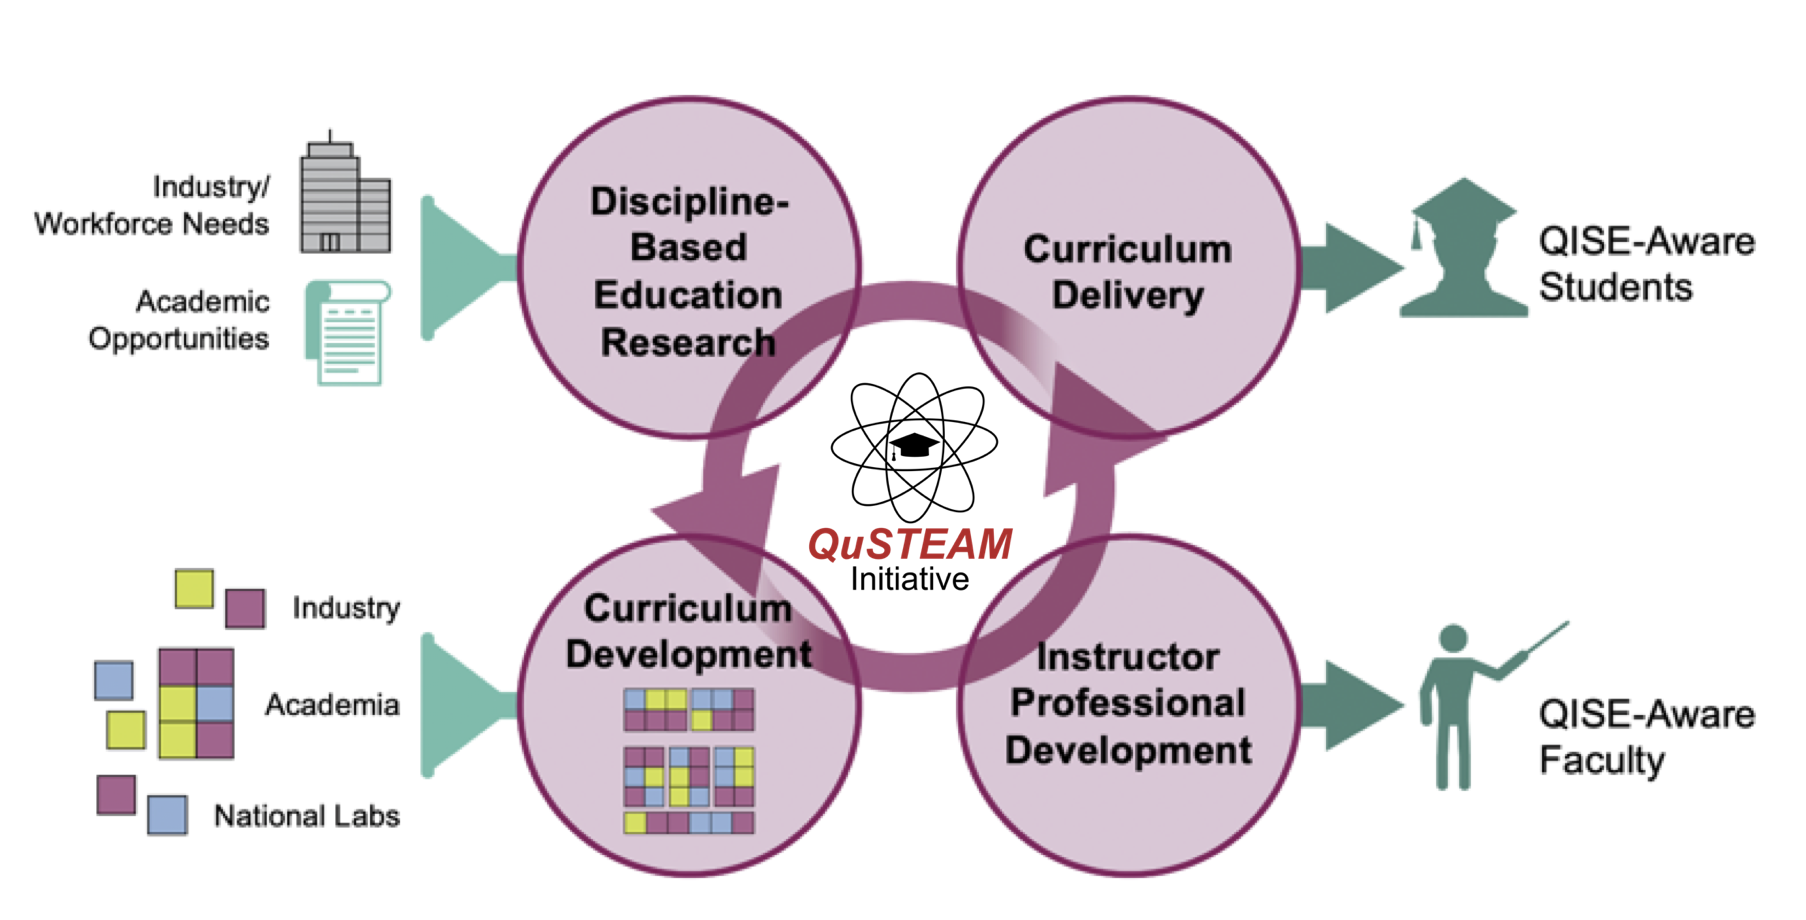
\includegraphics[width=0.7\linewidth]{qusteam.png}}

\vspace{6mm}

The reason why we believe the CCSE should be involved in planning this BSc program is that it has the necessary expertise to address several issues, such as

\begin{enumerate}
\item Lots of conceptual learning: superposition, entanglement, QIS and QT, etc. 

\item Connecting statistics and mathematics with ML methods

\item Linking ML algorithms with quantum ML.

\item Coding is indispensable. This is a central reason why the CCSE should be involved.

\item Experience with teamwork, project management, and communication are important and highly valued.

\item Experience with engagement with industry, public sector and priority to diversity through the Computational Science program and other activities at the CCSE.

\item Mentorship should begin the moment students enroll. The experiences with the Computational Science program developed at the CCSE will be of great value, as the activities of the KURT center.
\end{enumerate}

\noindent
\subsection*{Societal needs}

The program aims at addressing future societal needs, such as the
needs for specialized candidates (Master of Science, PhDs, postdocs),
but also the needs of people with a broad overview of what is possible
in QIS and QT. There are not enough potential employees in AI, ML, QIS
and QT. There is a clear supply gap.

A BSc degree with specialization is thus a good place to
start. Linking this with the Physics MSc program and the Computational
Science program and the study directions Computational physics and
Computational materials science, will offer our various research
fields top candidates as well as pointing to new research directions.

\subsection*{Study specializations in the BSc program}

The program could offer  three possible directions
\begin{enumerate}
\item Quantum information systems and quantum technologies

\item Artificial intelligence and machine learning in physics

\item Computational Physics
\end{enumerate}

\noindent
The students specialize in these directions in their last year of the BSc program.

There are several existing courses which can be included in this
program. There are also courses which need to be established. At the
CCSE we have the research and educational expertise to establish two
to three new courses in these directions. Most likely there are
potential teachers from other groups.

A separate application for establishing these courses follows. The
additional courses we propose are (these are suggestions and codes are
tentative) listed here. Note that we propose these courses as cloned
courses. We may consider extensions of these codes in order to offer
PhD variants as well.

The list here is tentative. Two of the courses, FYS4446 and FYS4447 have been taught as special topics since 2018 and we have already a large body of material.
This list is a mere suggestion.

\begin{enumerate}
\item Classical and quantum laboratory, needs to be established, perhaps by researchers at the Center of Materials Science (LENS group), FYS2440

\item Quantum computing and software, needs to be established. This can be organized together with OsloMet and Simula Research lab.

\item Quantum hardware, needs to be established, this can be organized together with OsloMet and Simula Research lab. 

\item Quantum computing and quantum machine learning, FYS3446/FYS4446 (cloned course, already developed by CCSE)

\item Advanced machine learning and data analysis for the physical sciences, FYS3447/FYS4447 (already developed by CCSE)
\end{enumerate}

\noindent
The last three courses are elective ones for the last semester of
study. Some of these courses can also be split into modules a 5 ECTS
or 7.5 ECTS.  There are obviously other course alternatives.  The
first year is identical with the BSc program \textbf{Physics and Astronomy}.

The table here is an example of a suggested path for a Master of Science project,
with course work the first year and thesis work the last year.


\begin{quote}
\begin{tabular}{llll}
\hline
\multicolumn{1}{l}{  } & \multicolumn{1}{l}{ 10 ECTS } & \multicolumn{1}{l}{ 10 ECTS } & \multicolumn{1}{l}{ 10 ECTS } \\
\hline
6th semester & Elective & Elective & Elective             \\
\hline
5th semester & FYS2160  & FYS3110  & Elective/FYS-STK3155 \\
\hline
4th semester & FYS2130  & FYS2140  & STK2100/FYS2440      \\
\hline
3rd semester & MAT1120  & FYS1120  & FYS3150              \\
\hline
2nd semester & MAT1110  & FYS12XX  & FYS13XX              \\
\hline
1st semester & MAT1100  & IN1900   & FYS11XX              \\
\hline
\end{tabular}
\end{quote}

\noindent
\subsection*{Description of Study directions}

The basic structure of the study directions could be

\begin{itemize}
\item Description of study directions with potential projects

\item Admission criteria

\item Learning outcomes

\item Program structure

\item Semester abroad

\item Career prospects

\item Teaching and examinations
\end{itemize}

\noindent
What follows are text proposals for these items.

\subsection*{Description of learning outcomes}

The power of the scientific method lies in identifying a given problem
as a special case of an abstract class of problems, identifying
general solution methods for this class of problems, and applying a
general method to the specific problem (applying means, in the case of
computing, calculations by pen and paper, symbolic computing, or
numerical computing by ready-made and/or self-written software). This
generic view on problems and methods is particularly important for
understanding how to apply available, generic software to solve a
particular problem.

Computing competence represents a central element
in scientific problem solving, from basic education and research to
essentially almost all advanced problems in modern
societies. Computing competence is simply central to further
progress. It enlarges the body of tools available to students and
scientists beyond classical tools and allows for a more generic
handling of problems. Focusing on algorithmic aspects results in
deeper insights about scientific problems.

The learning outcomes are subdivided in three general categories, knowledge, skills and general competence.

\subsection*{Study abroad and international collaborators}

Students at the University of Oslo may choose to take parts of
their degrees at a university abroad.

Students in this program have a number of interesting international
exchange possibilities. The involved researchers have extensive
collaborations with other researchers worldwide. These exchange
possibility range from top universities in the USA, Asia and Europe as
well as leading National Laboratories in the USA.

\subsection*{Career prospects}

Candidates who are capable of modeling and understanding complicated
systems in natural science, are in short supply in society.  The
computational methods and approaches to scientific problems students learn
when working on their thesis projects are very similar to the methods
they will use in later stages of their careers.  To handle large
numerical projects demands structured thinking and good analytical
skills and a thorough understanding of the problems to be solved. This
knowledge makes the students unique on the job market.

Career opportunities are many, from research institutes, universities
and university colleges and a multitude of companies. Examples
include IBM, Hydro, Statoil, and Telenor.  The program gives an
excellent background for further studies.

The program has also a strong international element which allows students to
gain important experience from international collaborations in
science, with the opportunity to spend parts of the time spent on
thesis work at research institutions abroad.


% ------------------- end of main content ---------------

\end{document}

